\documentclass[11pt]{article}
\usepackage{graphicx}
\graphicspath{ {images/} }
\begin{document}

\begin{titlepage}

\begin{center}
\begin{huge}
Swarm Visualiser - COS 301 Main Project
\\
Architecture Requirements and Software Architecture
\begin{small}
\\
Team: Dragon Brain
\\
Members:
\\
Matheu Botha u14284104
\\
Renton McInytre u14312710
\\
Emilio Singh u14006512
\\
Gerard van Wyk u14101263

\end{small}

\end{huge}
\end{center}
\end{titlepage}

\pagebreak

\tableofcontents

\pagebreak
\section{Vision of System}
The vision of the system, as expressed by the client, would be to create a standalone, fully functioning, experimental and teaching tool that brings to life, the functioning of a Particle Swarm Optimisation problem solver coupled to a real time graphical visualiser to display the workings of the Particle Swarm Optimisation problem solver to the user.

\section{Scope of System}
The Swarm Visualiser, as commissioned by Mr Christopher Cleghorn, has two fundamental responsibilities that are encapsulated within a single software program that is deployed to and used from a single computer at a time.

The first responsibility is to provide a underlying, adaptable and fully functioning Swarm Based Optimisation System that makes use of Swarm Based Optimisation algorithms such as the Particle Swarm Optimisation Model or PSO Model to solve problems. The problems that need to be solve are mathematical functions, of various dimensionality and domain.

The second responsibility, and the more important one, is to provide a real time graphical visualisation of the Swarm Based Optimisation Algorithm as it functions in terms of visualising all essential elements of the Swarm Based Optimisation Algorithm as it performs problem solving and then presenting this information to the user in a real time and understandable manner.

To this end, our system is ultimately responsible for providing both the underlying infrastructure in which the Swarm Based Optimisation Algorithm will operate but also for providing the interface infrastructure through which the user will access the underlying Swarm Based Optimisation Algorithm functionality.

\subsection{Extended Scope}
Below are some feature that extend on the core scope which would enhance the systems usability. The stretch goals are listed below.
\begin{itemize}
\item Functionality for a use to generate a predefined starting population for an algorithm in the form of a csv file and import it into the system.
\item Functionality to export the results of an algorithm to a csv file.
\end{itemize}


\section{Architectural Requirements}
\subsection{Scope}
In terms of the Architectural Scope of the project, we have a task that requires a minimal reliance on extremal frameworks and APIs. This is on account of the fact that our product is at its core a desktop application designed to be run in an isolated environment. Additionally, the focus on minimal interference requires that we design the system in such a manner that there is as low a possibility of bottlenecking as possible. As such, we will (as far as possible) minimize the technologies being used to standard C++ and OpenGL. Additionally, the system must be designed in such a manner that the Visualizer and the underlying Swarm Based Optimisation Algorithms are not tightly coupled. It should be easy to adjust one or the other without making adjustments throughout.
\subsection{Quality Requirements}
\paragraph{Performance}
Performance is arguably the most vital requirement in the system that in the Visualizer's functionality. It can be defined as follows:
\newline\textit{The amount of work accomplished in a measured time interval.}
\newline In our case, we are going to make use of reference to \textbf{latency} and \textbf{frames per second} as a measure of performance, where latency is defined as \textit{a time interval during which a response is achieved given some request} and frames per second, or fps, is defined as \textit{a measurement of how many unique consecutive images can be shown in a graphical context per second}. It should be noted that due to the graphical implications of our task, an important factor in performance is rendering resolution.
\paragraph{•}
As such, the following requirements are set:
\begin{itemize}
	\item The architecture of the design should be efficiently designed such that when a request is issued to the Visualizer, such as changing the objective function, there is a minimal latency involved in generating a response.
	\item The visualizer should be allow at least the following resolutions: 800x600, 1024x789, 1920x1080
	\item Given the maximum resolution 1920x1080, the Visualizer should be capable of running at a consistent 60fps or greater when being run using a mid-tier or above Graphical Processing Unit (for example).
	\item Given the fact that split-screen functionality is to be implemented, this must be done in a manner such that performance is not hindered dramatically (hence, do not render multiple full resolution images and shrink them post-rendering).
\end{itemize}

\paragraph{Scalability}
Scalability refers to the project's ability to handle a large workload for extended time periods and the methods through which this is dealt. Being an isolated application, the only workloads to be experienced are in terms of internal utilization. Hence, in terms of the task described, potential scalability issues lie within the task of assigning a large number of particles in a particular instance of running. 
\newline However, the system must still be capable of handling a large number of particles in order to achieve a satisfactory result. As such, the requirement in place is that the system should be capable of handling a large (with some upper limit based on hardware limitations) number of particles while still obtaining a good performance result. This will be achieved through effective use of object memory management and design patterns.

\paragraph{Flexibility}
Flexibility is a very important quality requirement for the system. Various pieces of the underlying PSO or Particle Swarm Optimisation system that the Swarm Visualiser is meant to be visualising are dependent on configuration parameters and pluggable components such as Objective Functions. It is important that the system be flexible enough so that users can modify the operational parameters of the system without having to perform major code changes, ideally without having to perform code changes at all.
\paragraph{•}
This is particularly important when you consider that the system should not depend heavily on hard-coded components like objective functions but must rather be able to switch to new ones as and when the client requires it.

\paragraph{Usability}
Usability is another important quality requirement. Ultimately, the system is meant to be used in some capacity as both an experimental tool and a tool for aiding in teaching. Both of these would therefore require that the system be fundamentally easy to use. Some degree of technical competence is assumed on the part of the users,but for the most part, interfacing with the system to access core functionality should not be unintuitive or frustrating. 

\paragraph{•}
An additional aspect of this usability is defined in terms of how usable the interface to perform modifications to the system must be. The system, as envisioned, is meant to be highly configurable and the means by which this is accomplished must be as simple as possible. 

\paragraph{•}
Although not strictly mandated, traditional values of usability design will be considered in order to deliver on a user-friendly interface that supports maximum usability without sacrificing functionality.
\subsection{Integration and Access Channels}
\paragraph{•}
The Swarm Visualiser or Particle Swarm Visualisation System that we are developing has very little in the way of integration requirements in terms of needing to interface and integrate with external services and programs. Rather, the client has expressed a desire for the system to function largely as a self-dependent and standalone system meaning that all of the functionality required by the system will be provided on-site by the program.

\paragraph{•}
That being said, the requirements for the system in terms of access channels is much more important. The client has specified that they wish for a single-point-of-access system. This translates to the provision of a single user interface that the client(s) will use to interact with and express the system's functionality. This single user interface must be designed such that it provides the graphical/visualisation requirements as specified as by the client, such as 4-screen display and support for various screen resolutions, but also must provide an interface through which the client can interact with and access the underlying system.

\paragraph{•}
Further provision for alternative deployment systems, beyond deployment of a single computer-based application, is limited due to the existing hardware demands that are contiguous to the performance requirements of the system.

\section{Architecture Patterns}
\subsection{Layered System}
\paragraph{•}
Why use a layered system?
\begin{itemize}
\item It simplifies the design considerably.
\item It enables different team members to work on different components without being dependant on the progress of the other components.
\item It enables different team members to work at various levels of abstraction.
\item It supports the portability of software artefacts.
\end{itemize}
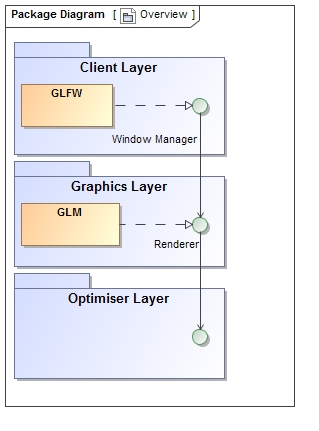
\includegraphics{Overview}
\subsection{Optimiser layer}
The Optimiser layer will encompass all the functions performed by the generic interchangeable optimisation algorithm that is being visualised. The graphics layer will request information from the optimiser layer at regular intervals in order to render the particles representing the optimiser's current sample points onto the current fitness landscape. The optimiser will act according to what type of optimiser has been selected by the user.
\subsection{Graphics Layer}
The Graphics Layer is responsible for using requests from the client layer and the output of the Optimiser Layer to render the scene and pass it back to the client interface.
\subsubsection{Approach}
\paragraph{•}
Graphics engine are not traditionally developed under the traditional OO approach. This is mainly due to various performance issue that graphical processing encounters with Object Orientation. Instead a more effective approach is data-driven design. Its basic premise is simple: construct your code around the data structures, and describe what you want to achieve in terms of manipulations of these structures.

\paragraph{•}
Functional Reactive Programming is one such programming style that promotes data driven design. There are 3 common divisions of FRP:
\begin{itemize}
\item Discrete - Formulations such as Event-Driven FRP and Elm require that updates are discrete and event-driven. These formulations have pushed for practical FRP, focusing on semantics that have a simple API that can be implemented efficiently in a setting such as robotics or in a web-browser.

In these formulations, it is common that the ideas of behaviors and events are combined into signals that always have a current value, but change discretely.

\item Continuous - The earliest formulation of FRP used continuous semantics, aiming to abstract over many operational details that are not important to the meaning of a program. The key properties of this formulation are:
\begin{itemize}
\item Modeling values that vary over continuous time, called "behaviors" and later "signals".
\item Modeling "events" which have occurrences at discrete points in time.
\item The system can be changed in response to events, generally termed "switching."
\item The separation of evaluation details such as sampling rate from the reactive model.
\end{itemize}

This semantic model of FRP in side-effect free languages is typically in terms of continuous functions, and typically over time.
\end{itemize}
\subsubsection{Unit Testing}
\paragraph{•}
With a data orientated approach, your aim is to create a compartment of code that contains functions that will typically only have a single use. i.e. no decisions will ever be made in the functions, the decisions will be made the the graphics engine and the graphics engine will use this grab bag of functions to execute whatever it has decided. This approach allows for powerful, comprehensive unit testing due to the fact that the functions are minimalistic in nature. This is especially useful when debugging a graphical applications as you can unit test an image output, but if you have a comprehensive unit testing backbone for the functions then it can make it easier to see logical mistakes.
\paragraph{•}
The basic premise of data orientated design is to design the code around the data, instead of abstracting the data behind models. While this may seem counter intuitive it is still possible to achieve a familiar level of abstraction while still making use of the performance increases that come with the approach.
\subsection{Client Layer}
The client layer will handle Graphical User Interface elements that the software user will interact with, and will present the output of the Graphics layer(and implicitly the Optimiser layer) to the user. The user will also use the client layer to set parameters of the optimiser layer to determine which fitness landscape will be used, which optimisation algorithm will be used, and also let the user set the optimiser's parameters.
\subsection{Technologies}
\subsubsection{OpenGL}
OpenGL was chosen as the graphics engine due to the fact that it will work cross-platform, as opposed to DirectX, and many of the CIRG members run Linux machines, as per client stipulations. Since this program is primarily going to be used by them it makes sense to cater for the target market. 
\subsubsection{Fruit}
Fruit is a dependency injection framework for C++, loosely inspired by the Guice framework for Java. It uses C++ metaprogramming together with some new C++11 features to detect most injection problems at compile-time. It allows to split the implementation code in "components" (aka modules) that can be assembled to form other components. From a component with no requirements it's then possible to create an injector, that provides an instance of the interfaces exposed by the component. This is a good option for the DI framework as unlike other c++ DI frameworks most of the checks are done at compile-time to try catch the errors early. Another bonus is that the syntax is similar to jUnit so it will be more comfortable to work with initially.
\subsubsection{GLEW}
The OpenGL Extension Wrangler Library (GLEW) is a cross-platform open-source C/C++ extension loading library. GLEW provides efficient run-time mechanisms for determining which OpenGL extensions are supported on the target platform. OpenGL core and extension functionality is exposed in a single header file. GLEW has been tested on a variety of operating systems, including Windows, Linux, Mac OS X, FreeBSD, Irix, and Solaris.
\subsubsection{GLM}
The graphics layer will make use of the OpenGL Mathematics(GLM) framework. This is a light-weight, optimized mathematics framework that handles matrix manipulations and shader control.
\subsubsection{GLFW}
The client Layer will make use of the GLFW. GLFW is an Open Source, multi-platform library for creating windows with OpenGL contexts and receiving input and events. It is easy to integrate into existing applications and does not lay claim to the main loop.
\subsubsection{CMake}
CMake is an open-source, cross-platform family of tools designed to build, test and package software. CMake is used to control the software compilation process using simple platform and compiler independent configuration files.
\subsubsection{Fraps}
Fraps is a universal Windows application that can be used with games using DirectX or OpenGL graphic technology. For our purposes it will be used as the benchmarking software as it can how how many Frames Per Second (FPS) you are getting in a corner of your screen.  Perform custom benchmarks and measure the frame rate between any two points. It can also save the statistics out to disk and use them for your own reviews and applications. It also has useful Screen Capture Software as well as Realtime Video Capture Software which can be useful for demoing purposes.

\end{document}
